\newpage
\section{Задание 5.}

Найти объем тела, ограниченного поверхностями. Рисунок желателен. Па-
раметры считать положительными.
$$\left(x^{2}+y^{2}+z^{2}\right)^{3}=a^{6}\sin^{2}\left(\frac{\pi z}{\sqrt{x^{2}+y^{2}+z^{2}}}\right)$$
Тут напрашиваются сферические координаты. Сделаем переход.
$$
\begin{cases}
    x=r\sin{\theta}\cos{\phi}\\
    y=r\sin{\theta}\sin{\phi}\\
    z=r\cos{\theta}
\end{cases} \Rightarrow \quad \left(r^2\right)^{3}=a^{6}\sin^{2}\left(\frac{\pi r\cos{\theta}}{\sqrt{r^2}}\right) \Rightarrow \quad r^6 = a^6\sin^2\left(\pi\cos{\theta}\right) \quad \big/ \sqrt[6]{\text{     }}$$
$$r = a\sqrt[3]{\sin\left(\pi\cos{\theta}\right)}$$
Теперь мы знаем, что $r\in\left(0, a\sqrt[3]{\sin\left(\pi\cos{\theta}\right)}\right)$. Значит, мы можем записать интеграл.
$$\int_0^{2pi}\int_0^{\pi}\int_0^{a\sqrt[3]{\sin\left(\pi\cos{\theta}\right)}} \,dV = \int_0^{2pi}\int_0^{\pi}\int_0^{a\sqrt[3]{\sin\left(\pi\cos{\theta}\right)}} r^2\sin{\theta}\,dr\,d\theta \, d\phi =$$ 
$$=\int_0^{2pi}\, d\phi \int_0^{\pi} \sin{\theta}\,d\theta \int_0^{a\sqrt[3]{\sin\left(\pi\cos{\theta}\right)}} r^2\,dr = \int_0^{2pi}\, d\phi \int_0^{\pi}\dfrac{a^3}{3} \sin{\theta}\sin\left(\pi\cos{\theta}\right)\,d\theta = $$
\begin{center}    
    Сделаем замену переменной, пусть $u = \pi\cos{\theta}$, тогда $du = -\pi\sin{\theta}\,d\theta \Rightarrow -\dfrac{1}{\pi}\,du = \sin{\theta}\,d\theta$ 
    Насчет границ интегрирования: $\pi\cos{0} = \pi, \pi\cos{\pi} = -\pi$
\end{center}
$$\int_0^{2pi}\, d\phi \int_{\pi}^{-\pi}-\dfrac{a^3}{3\pi} \sin{u},du = \int_0^{2pi}\, d\phi \int_{-\pi}^{\pi}\dfrac{a^3}{3\pi} \sin{u},du \Rightarrow$$
\begin{center}    
    Синус нечетная функция, поэтому мы получим ноль. Но объем фигуры не может быть нулем, она просто симметрична относительно плоскости $XY$. Тогда поменяем границы интегрирования и удвоим интеграл.
\end{center}
$$\Rightarrow \int_0^{2pi}\, d\phi \int_{0}^{\pi}\dfrac{2a^3}{3\pi} \sin{u}\,du  = \dfrac{2a^3}{3\pi}\int_0^{2pi} \left[-\cos{u}\right]_0^{\pi}\, d\phi = \dfrac{2a^3}{3\pi}\int_0^{2pi} 2\, d\phi = \dfrac{2a^3}{3\pi} \cdot 4\pi =\boxed{\dfrac{8a^3}{3}}$$

\begin{figure}[h!t]
    \centering
    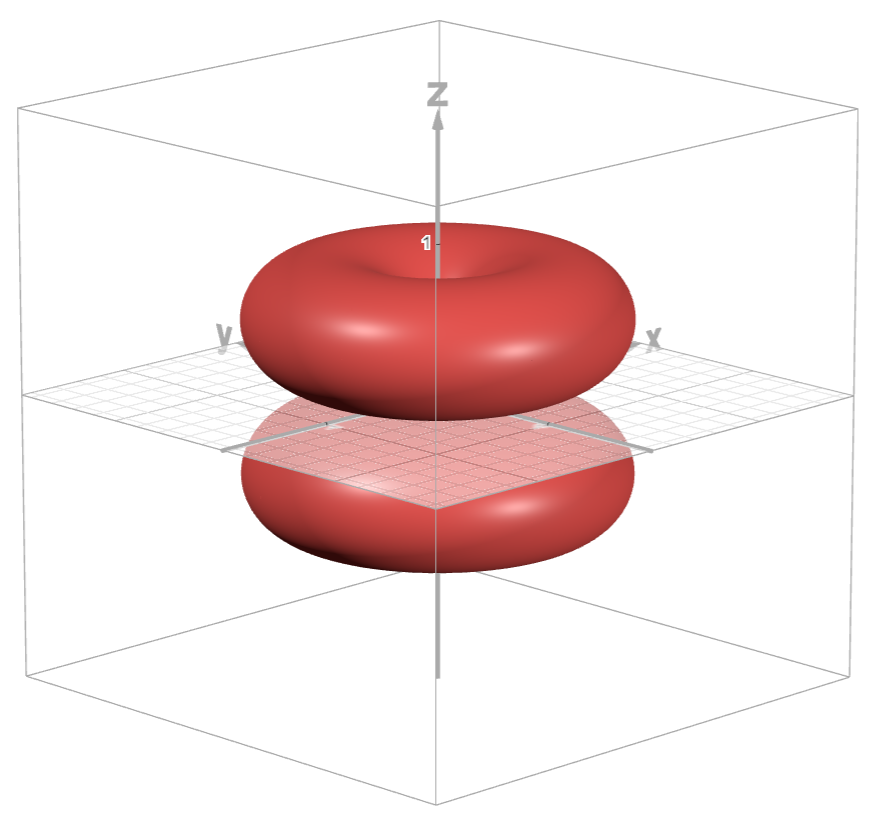
\includegraphics[width=0.5\linewidth]{Task5/Figure_shape.png}
    \caption{Задание 5. Изображение фигуры. \underline{\href{https://www.desmos.com/3D/hq9g3zataj}{(Desmos)}}. }
\end{figure}